\documentclass[letterpaper,12pt,oneside]{book}
\usepackage[top=1in, left=1.25in, right=1.25in, bottom=1in]{geometry}
%-----------------------__--------
%https://es.overleaf.com/project/642e50d937469ff17340bdc4
% Tesis UNAM https://tex.stackexchange.com/questions/234265/unam-thesis-title-page-portada-tesis-unam

\usepackage{pdfpages}
\usepackage{lipsum}

\usepackage[T1]{fontenc}
\usepackage[utf8]{inputenc}
\usepackage[spanish,es-nodecimaldot,es-tabla]{babel}
\usepackage{graphicx}
\usepackage{tikz}
\usepackage{setspace}


%Subfiguras
\usepackage{caption}
\usepackage{subcaption}

% Para referencias 
\usepackage{hyperref}
\usepackage{apacite}
\usepackage{url}


\title{E-CARDIAC: La evolución hacia un modelo concurrente y paralelo}

\begin{document}
	\frontmatter
	%\maketitle

    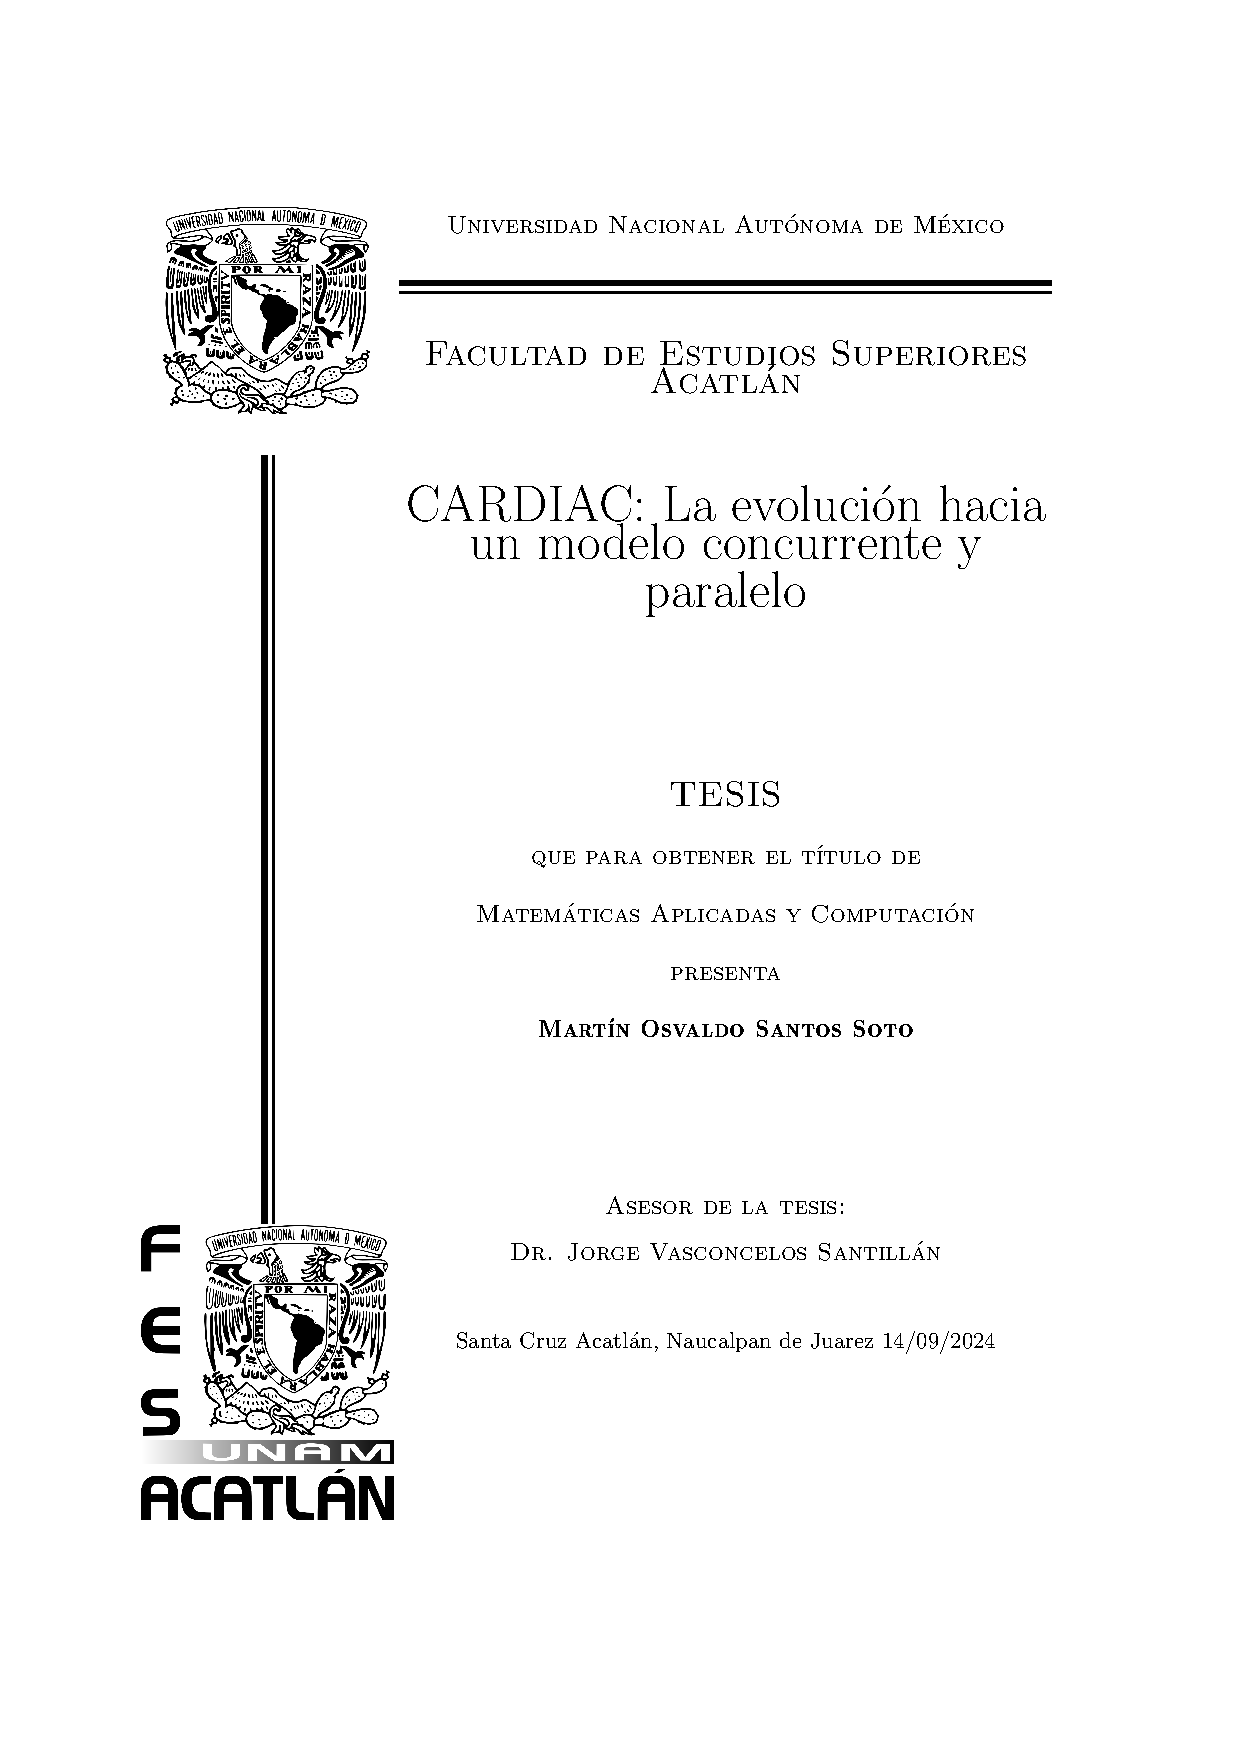
\includepdf{cover.pdf}

%---------------------------------
\chapter*{}
\begin{flushright}%
  \emph{A la facultad que me permitió crecer...}
  \thispagestyle{empty}
\end{flushright}

\chapter{Agradecimientos}
%\spacing{1.5}%\doublespacing

\chapter{Abstract}

\chapter{Introducción}

	Hoy en día tenemos multitud de aparatos electrónicos que pueden ser llamados computadoras; celulares, laptops, tabletas, relojes inteligentes, y un sin fin más. 
	Estos aparatos pueden ser llamados así siempre que sean  capaces de resolver operaciones aritméticas y lógicas de manera automática, al menos en la definción
	más aceptada que recoge el diccionario de Cambridge(dado que la palabra de origen es anglosajona en este contexto),
	por que sin analizamos más puntualmente el termino ``computadora''  notaremos que el origen de la palabra es anterior a las computadoras
	tal cual las conocemos hoy día, por ejemplo las primeras nociones de ``computadoras''  eran referidas a mujeres de los años 1930 en estados unidos
	que trabajaban en la NASA y realizaban cálculos manuales. Si analizamos la historia notaremos que el avance cientifico en cuanto a maquinas
	que pudieran automatizar tareas que realizaba la humanidad estaban centrados en las calculadoras, había que hacer los calculos matematicos menos
	complejos, ya sea con la invención de maquinas o bien con tecnicas como los logaritmos y las tablas de multiplicar que se tenian
	para consultar más rapidamente operaciones complejas y repetitivas; de ahí su amplia relación, hasta en el nombre, de las computadoras y las calculadoras.
	
	%%https://www.smithsonianmag.com/science-nature/history-human-computers-180972202/
	
	Está relación se hace muy palpable regresando al siglo 19, para ir un poco a los origenes de la computación,
    más precisamente en el año 1830 el entusiasta charles Babbage había desarrollado una maquina llamada ´´Diferential Engine''
	que resolvía ecuaciones matemáticas, una calculadora potente si lo queremos ver desde otra perspectiva. Pero años después también estuvo diseñando e intentando 
	construir por mucho tiempo su ´´Analytical Engine'', que aunque fue imposible de construir por la tecnología de la epoca, ya fue pensada como una computadora
	de proposito general, en el sentido que podía hacer calculos y resolver operaciones lógicas además de que era una maquina que se podía programar,
	cumpliendo así todos los puntos básicos para poder ser considerada como una computadora, pero lamentablemente no pudo llegar a ver la luz de la mano
	de su creador.
	
	Podríamos ir aún más atrás en el tiempo con el desarrollo de las primeras ''calculadoras´´, que son las predecesoras de las
	computadoras actuales, pero regresemos al presente. Cuando vemos alguno de nuestros dispositivos ¿analizamos como es que funcionan por dentro? ¿ como podemos enviar mensajes de texto mientras escuchamos la canción del momento?
	usualmente la respuesta es ´´No'', que no es necesariamente una respuesta mala, como personas en nuestro día a día no podemos detenernos a analizar cada artefacto que tengamos cerca o usemos, a pesar de que sería muy útil saberlo
	si funciona el aparato es todo lo que necesitamos saber, después de todo hay muchas cosas más importantes
	a las cuales prestar atención. Sin embargo, para los profesionales del área de la computación o tecnología en general, así como a aquellos apasionados
	por estás tecnologías son preguntas que no pueden faltar en nosotros. Y es que incluso si tu trabajo es el desarrollo web o
	el diseño de gráficas entender las razones por las cuales tu computadora o las computadoras para las cuales desarrollas programas pueden hacer computos
	en paralelo o tener la potencia que tienen es fundamental para poder optimizar tus desarrollos, que decir si tu trabajo es la parte del hardware, en ese
	caso debes estar totalmente involucrado con el funcionamiento interno de las computadoras.
	Más aún, considero que al igual que en toda disciplina la historia de la misma o de los artefactos que estudia está debe ser conocida por
	los apasionados a está disciplina y sobretodo los profesionales, dado que hay que entender como ha sido la evolución, lo que ha cambiado
	y aquello que a pesar de los años sigue vigente y la razón por la cuál sigue vigente.
	
	Pero entender la historia de la computación podría parecer tedioso o complicado, 
	 a pesar de que quizá la historia de las computadoras modernas es corta hablando del tiempo
	de los humanos, es larga a nivel de la evolución que ha habído en los últimos 80 años, esto puede parecer tedioso, si yo me pregunto como funciona una computadora
	de hoy ¿será igual que las de hace 30 años con Windows 98? o aún peor ¿como será de diferente con aquellos monstruos gigantes que sólo operaban los eruditos
	de la computación en los años 50? o preguntas más especificas como  ¿Que tiene que ver mi procesador Intel con 5 nucleos y una computadora con un transistor? ¿por que 	
	antes no se podía hacer computo en paralelo? Todas estás preguntas son naturales, y en mi opinion hacer una relación directa entre la historia y el funcionamiento de
	las computadoras nos puede dar un conocimiento más amplio y sobre todo el contexto historico puede resolvernos
	muchas dudas del por que se tomaron deciciones sobre el diseño o funcionamiento de las computadoras que quizá ahora para nosotros no parezcan las mejores.
	
	Cuando yo me hice estás preguntas hace algunos años en los principios de mi carrera universitaria me encontre con algunos problemas, la barrera del idioma, dado
	que la lingua franca de la computación es en inglés muchos escritos están en ese idioma, y aunque hay muchos traducidos, otros más, en especial aquellos más 
	relacionados a partes antiguas de la computación no lo estan. Otro, quizá el más imporante, es que tu puedes seguir la historia de la computación en diversos 
	documentos, algunos	con más detalles tecnicos que otros, pero que al final no se van a centrar en el funcionamiento de las computadoras, y en la otra mano tenemos los 
	manuales
	o libros sumamente tecnicos acerca del funcionamiento de estás, de como funciona el paralelismo, de las necesidades y utlidad del sistema operativo que
	son realmente dificiles de leer para un estudiante que va empezando en la carrera. Este problema no es nuevo, ya se habían enfrentado a el no solo muchos
	estudiantes desde la aparición de la computación, sino también muchas instituciones y empresas que querían que más personas aprendieran a usar una computadora,
	y es aquí dónde podemos ver lo relevante el contexto historico, en los años 50 y 60 si querias usar una computadora tenías que entender muy bien el como funcionaba,
	no había una interfaz gráfica y un Sistema Operativo que hiciera el trabajo rudo por ti, tenías que entender como se movía por dentro la computadora para
	poder programar y resolver tus problemas. Es aquí, en este periodo historico, más precisamente en los años 60, cuando varias compañias e instituciones
	educativas comienzan lanzan ciertos modelos, manueales y kits para que los estudiantes aprendieran a usar computadoras tales como Little Man Computer lanzado por
	Madnick en los años 60, que básicamente era un kit de papel con un manual, una computadora de papel como se les ha llamado, en la cual tu como estudiante
	podías ver como eran las ejecuciones del código que habías escrito, y como eso se materializaba en una respuesta a tu problema inicial. Y aunque
	es apasionante y algo controvertido LMC no nos centraremos en el, sino en la contemporanea CARDIAC(CARDboard Illustrative Aid to Computation) desarrollada
	por Bell Labs de la mano de David W. Hagelbarger, que es
	muy similar a lo descrito sobre LMC, pero con su propio lenguaje y su porpia arquitectura. Volvemos a la parte del contexto historico, en aquellos tiempos
	las computadoras eran ordenadores gigantes y conseguir tiempo para usarlos era realmente dificl, comprarlos directamente imposible para las personas
	comunes, entonces la solución que encontraron para que los estudiante pudieran practicar es la creación de estos kits con computadoras de papel, que los
	preparaban  para cuando pudieran usar una computadora ´´de verdad''.
	
	Eso quizá nos pueda parecer una simple clase de historia de la computación, pero no lo es, CARDIAC sigue siendo muy útil y es de hecho la respuesta que encontre
	a mis preguntas sobre como entender a las computadoras, respuesta que encontré en una clase de programación paralela y concurrente en la cúal CARDIAC
	fue fundamental para entender varios conceptos. También hay que entender que con CARDIAC no te vas a volver un experto en el funcionamiento de las computadoras,
	el punto es entenderlas de una forma clara de modo que tengas las bases para entonces si ponerte a leer uno de esos manuales gigantes sobre sistemas
	operativos y arquitectura de computadoras con muchisimos conceptos técnicos, los cuales si no tienes cierto conocimiento de base te pueden desbordar.
	
	Aún con todas estás ventajas de CARDIAC, las limitaciones son evidentes, fue construida en el año 1968, no es apta para la concurrencia ni el paralelismo, o 
	incluso un computo distribuido, de aquí que las mentes brillantes que están en el mundo de la computación en los años posteriores han seguido haciendo
	modelos similares como MARIE a CARDIAC o directamente evolciones de ella como TIMBA, algunos más tecnicos que otros, varios incluso en español, aunque
	la mayoría en inglés, y estas creaciones son necesarias, las inquietudes no se iban a pausar por 40 años, han seguido y las segurian habiendo y encontraremos
	la forma de solucionarlas o al menos de acercarnos lo más posible. Al adentrarme más en estos modelos me di cuenta que los que más se acercaban a mi concepción
	de un buen modelo que explicará el funcionamiento de computadoras más avanzadas se volvían más tecnicos, como el desarrollo mexiano de 8-bit a complete Design, 
	que es un gran trabajo, pero que termina siendo bastante tecnico y los demás que no son tan tecnicos caen un poco en ser bastante similares a CARDIAC, lo cúal no 
	es malo, e incluso tiene muchas ventajas, pero no es lo que yo esperaba o más bien, la visión que yo tenía. Es en esté punto en el que decidi empezar este
	proyecto de investigación para explicar como funcionan las computadoras de una forma simple y didactica para aquellos estudiantes que van empezando la carrera,
	tomando como base el increible desarrollo de CARDIAC y llevandola unos pasos más allá en nivel de arquitectura para que sea capaz de explicar
	la computación concurrente y paralela. Con un enfoque particular que lleve al lector a ver las necesidades de hardware y software que hacen crecer a CARDIAC,
	pero que también, de una forma didactica, el lector entienda no solo los cambios que hubo en las computadoras en los últimos 60 años, sino
	las necesidades que llevaron a esos cambios, y en ese mismo camino aprovechar para situarse en el contexto historico de la epoca en que esos
	cambios se hicieron tangibles en las computadoras, esto dará mucha claridad del por que algunos cambios tardaron tanto en llegar y otros fueron bastante veloces.
	
	
	Más allá del recorrido en la construción y diseño de modelos ´´evolucionados'' de CARDIAC para computación paralela y concurrente el texto se verá acompañado,
	tal como la clasica CARDIAC distribuida por Bell Labs, con un kit que incluye un programa que contendra tres maquinas virtuales para cada
	modelo de CARDIAC, con la diferencia de que estas maquinas virtuales ya no serán en papel, sino interfaces gráficas para uso en computadoras de escritorio.



\tableofcontents
\listoffigures

\mainmatter

\chapter{Marco Teórico} %


\section{Inicios de la computación}
	\subsection{Primeros automatas}
	% Breve historia de como se fue desarrollando la computación desde los inicios hasta llegar a automatas(1950)
	\subsection{Primeras computadoras}
	%1950-1970
	\subsection{Nacimiento de CARDIAC}
	%El como nace el modelo para dar claridad a los trabajadores de ATT
	\subsection{Evolución hasta la actualidad}
   
\section{Arquitecturas de computadoras}   
   
\subsection{Modelo concurrente}

\subsection{Modelo paralelo}


\chapter{Metodología}  %
	\section{Necesidad de operaciones concurrentes}
	
	 \section{Evolución hacia el paralelismo}

\chapter{Resultados}  %


\chapter{Conclusiones}

%\bibliographystyle{humannat}
%\bibliography{references}

%\backmatter%@sglvgdor


\end{document}

